\needspace{20\baselineskip}
\section{Costos}

\begin{table}[H]
\centering\footnotesize
\caption{Costo de una mochila de prototipo con piezas de mostrador en México (precios del 9 de noviembre
de 2026~\cite{unit}). Con tarjetas de desarrollo no cumple la meta de masa: sirve para validar, no para montar.}
\label{tab:costos}
\rowcolors{2}{SoftGray}{white}
\begin{tabularx}{\textwidth}{@{}>{\raggedright\arraybackslash}X r r@{}}
\toprule
\rowcolor{TableHead} \textbf{Pieza} & \textbf{Con matriz $8\times8$} & \textbf{Con matriz $32\times24$} \\
\midrule
Matriz térmica (AMG8833 o MLX90640) & 599 & 1\,100 \\
Radio y procesador (XIAO nRF52840) & 248 & 248 \\
IMU (MPU6050) & 87 & 87 \\
Batería LiPo de 40~mAh & 41 & 41 \\
Dos LED ultravioleta (paquete de 100: 281) & 6 & 6 \\
Tarjeta, base y adhesivo (estimado) & 50 & 50 \\
\midrule
\textbf{Total por mochila (MXN)} & \textbf{1\,031} & \textbf{1\,532} \\
Equivalente a 18.8 MXN por dólar & 55 USD & 81 USD \\
\bottomrule
\end{tabularx}
\end{table}

Para la demostración del curso solo falta comprar la matriz térmica (599~MXN) y los LED
ultravioleta (281~MXN): la DE10-Lite y el ESP32 ya se tienen. El insecto cuesta de 2 a 15~dólares
por ejemplar en Estados Unidos; no se encontró un precio verificable en México.

\begin{figure}[H]
\centering
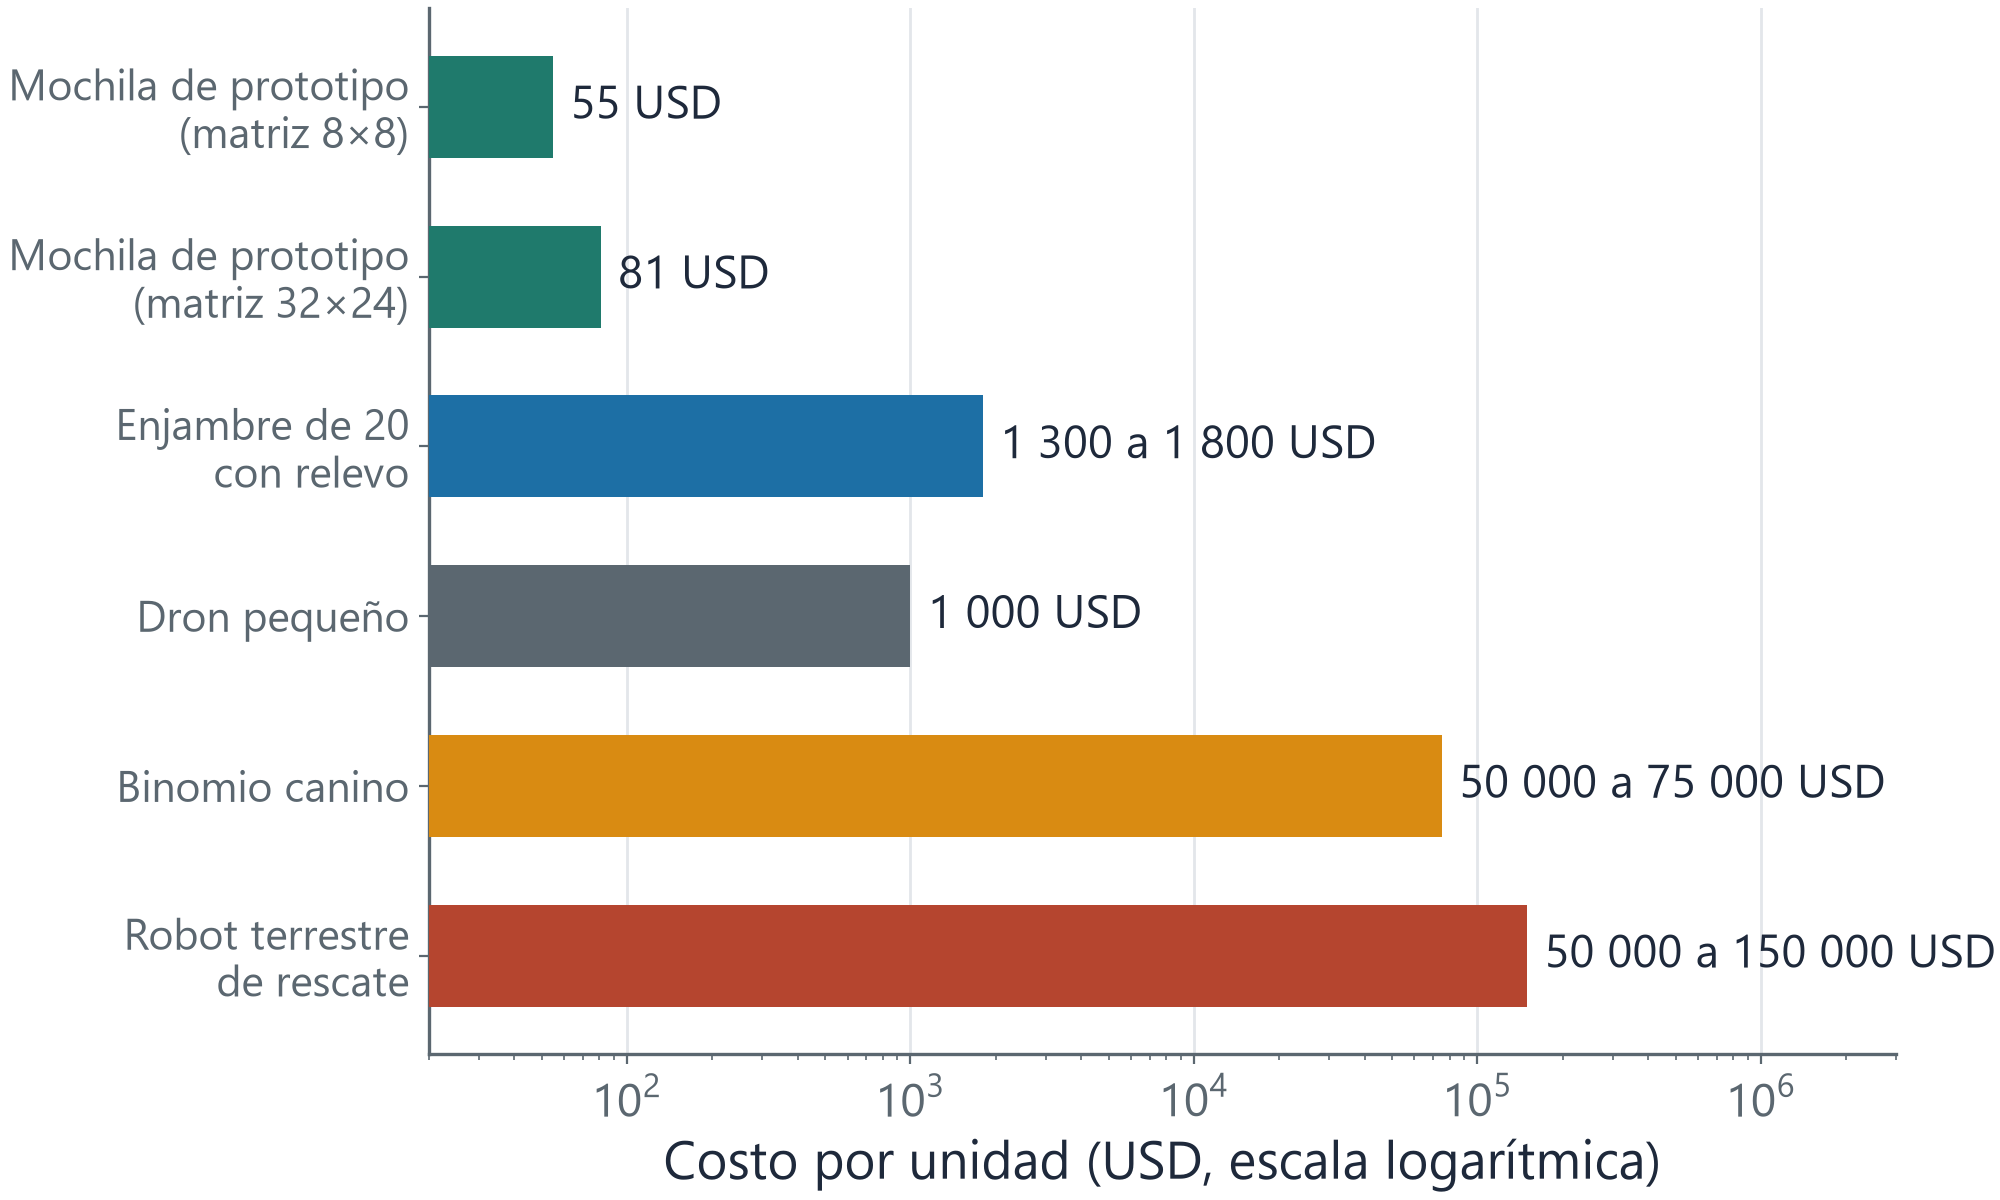
\includegraphics[width=0.72\textwidth]{figs/costos.png}
\caption{Costo por unidad frente a las alternativas. El enjambre de 20 con relevo es una estimación propia
(veinte mochilas más un nodo de radio). Fuentes: \cite{unit,murphy2021,sdf}.}
\label{fig:costos}
\end{figure}

Un enjambre completo cuesta entre 30 y 100 veces menos que un binomio canino o un robot de
rescate, pero la comparación tiene tres salvedades. No son sistemas equivalentes: el perro
encuentra personas y el biobot todavía no lo ha hecho en campo. El costo por unidad oculta la cría, el
personal que monta las mochilas y los permisos. Y la vida útil de cada unidad es corta. El dato
honesto es el costo por hora de búsqueda, que solo se conocerá con pruebas.

\needspace{14\baselineskip}
\section{Practicidad}

La pregunta práctica es si un rescatista podría usarlo. La tabla~\ref{tab:practicidad} cruza lo que
exige el campo con lo que el diseño ofrece.

\begin{table}[H]
\centering\footnotesize
\caption{Requisitos del campo y respuesta del diseño.}
\label{tab:practicidad}
\rowcolors{2}{SoftGray}{white}
\begin{tabularx}{\textwidth}{@{}>{\bfseries\raggedright\arraybackslash}p{3.5cm} >{\raggedright\arraybackslash}X >{\raggedright\arraybackslash}p{4.6cm}@{}}
\toprule
\rowcolor{TableHead} Lo que exige el campo & Cómo responde el diseño & Lo que falta \\
\midrule
Arrancar en menos de 2~min: los rescatistas se van si tarda más~\cite{murphy2004} & La mochila no se configura: se enciende y se suelta el insecto & Medir el tiempo real de preparación \\
No añadir operadores & Nadie pilotea; la estación solo recibe alertas & Probar con rescatistas \\
Sesiones cortas: 45~min en Myanmar~\cite{htx2025} & Autonomía estimada de 4~h & Medir el consumo del prototipo \\
Entrar en rendijas & Insecto de 1.3~cm; mochila de perfil bajo & La matriz térmica mide 5~mm de alto: hay que probar el paso \\
Funcionar con calor y con frío & Solo entre 22 y 30~\textdegree C & Sensor de CO$_2$ para el calor; caja térmica para el transporte \\
Avisar a través del escombro & Radio de menos de 1~GHz con relevo en el boquete & Medir el alcance: nadie lo ha publicado \\
Decir dónde cavar & Entrada conocida, navegación inercial y baliza & Probar el error real \\
Recuperar el equipo y los insectos & Mochilas numeradas; solo machos; conteo de entrada y salida; refugio y faro en el boquete (sección~\ref{sec:regreso}) & En simulación vuelve de \regTrampaDos{} a \regFaroDos~\% en dos horas; con insectos no se ha probado \\
Cumplir la ley & Pruebas en recinto cerrado & Un despliegue real exige autorización: ver la sección~\ref{sec:etica} \\
\bottomrule
\end{tabularx}
\end{table}

\textbf{Cómo se usaría.} El perro marca una zona. El rescatista coloca un relevo de radio en el
boquete, enciende de diez a veinte mochilas y suelta los insectos. Durante 45 a 60~minutos no hace
nada con ellos. Si una mochila alerta, la estación muestra qué insecto fue, por dónde entró y cuánto
caminó. El rescatista confirma con una cámara o con el perro antes de mover una losa. Una búsqueda
sin alertas no descarta que haya alguien: el sistema sirve para encontrar, no para dar por vacía una zona.

\textbf{Lo que el insecto impone.} No se puede contar con él por debajo de unos 20~\textdegree C ni por
encima de 34~\textdegree C; el CO$_2$ concentrado lo anestesia en segundos; bajo el agua sobrevive
minutos; con la mochila se endereza solo entre el 31 y el 82~\% de las veces, según el diseño. Son límites del
animal, no del circuito, y definen dónde el sistema no debe usarse.
